\section*{Math 202A - HW10 - Dan Davison - \texttt{ddavison@berkeley.edu}}

\begin{mdframed}
  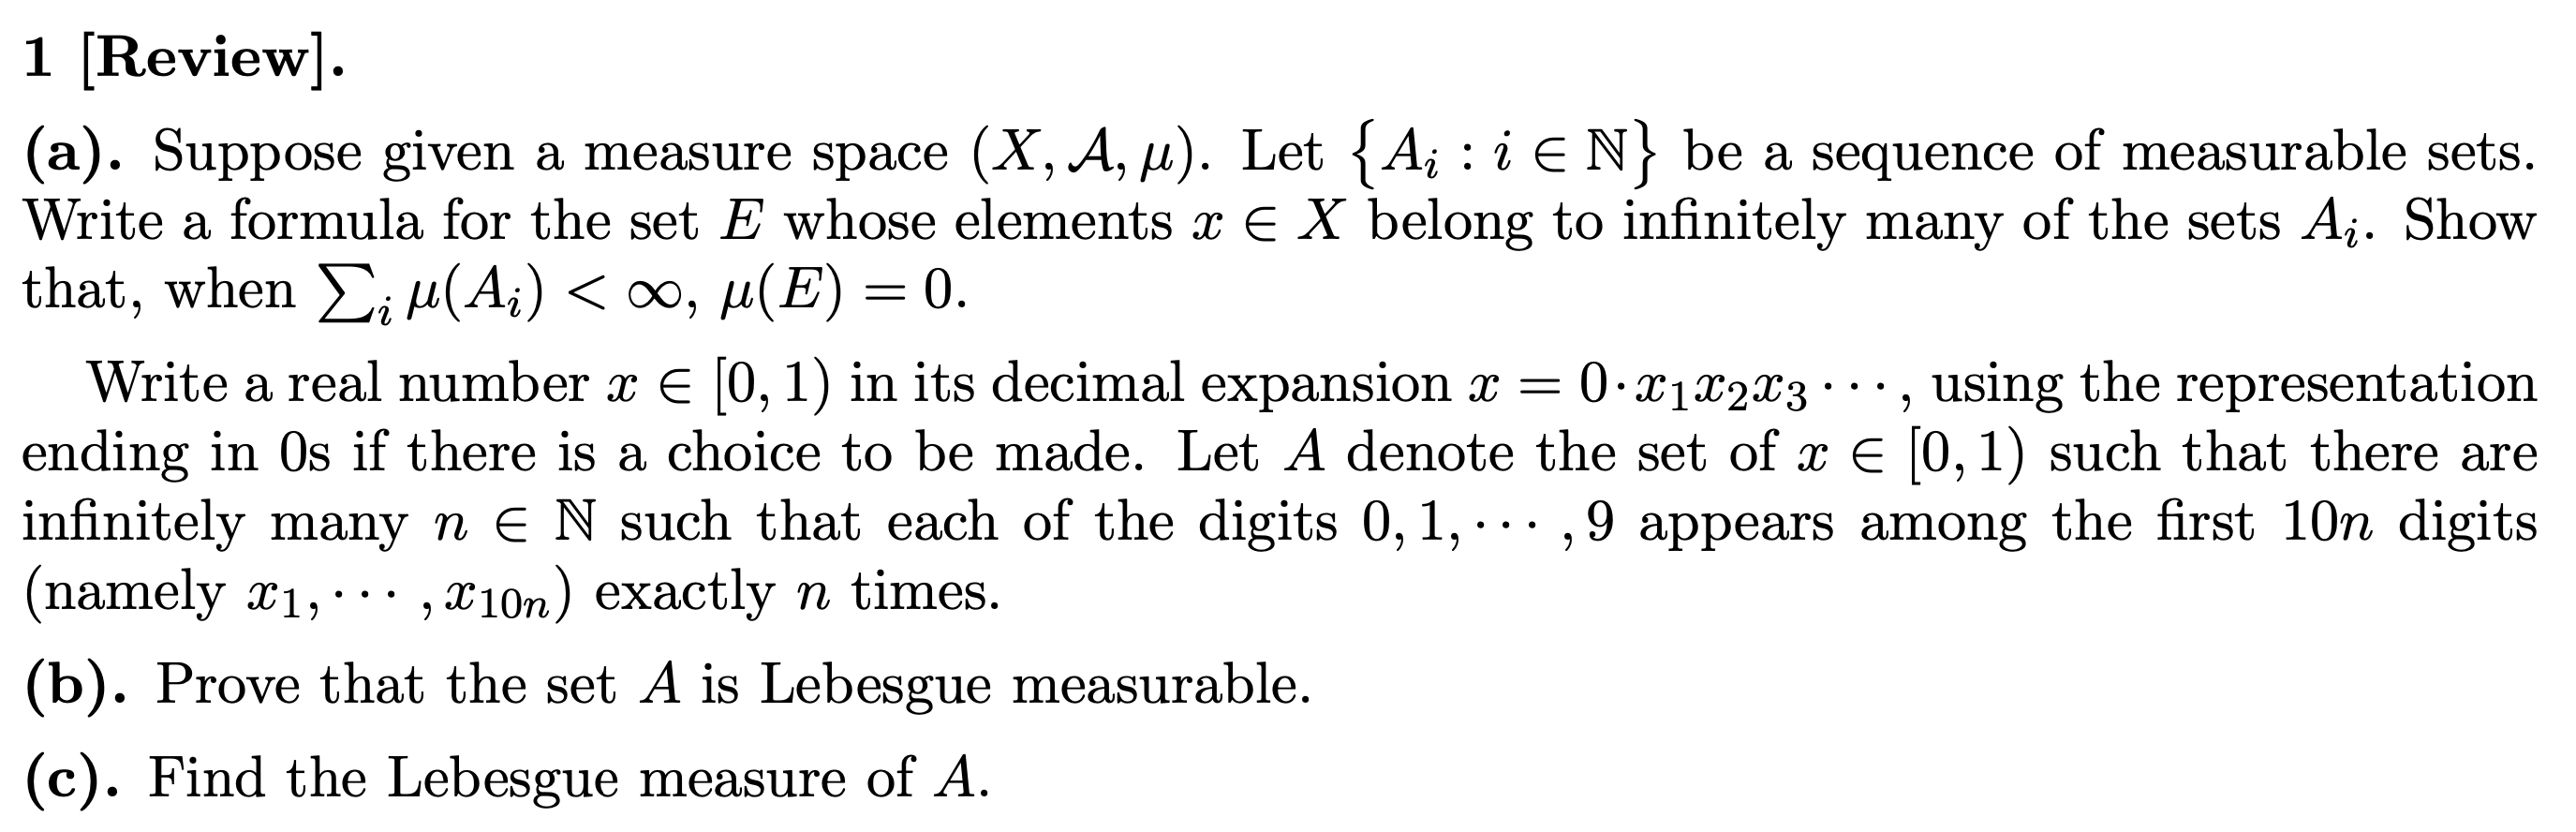
\includegraphics[width=400pt]{img/analysis--berkeley-202a-hw10-7127.png}
\end{mdframed}

\begin{enumerate}[label=(\alph*)]
\item ~\\

The set $E$ whose elements belong to infinitely many of the sets $A_i$ is
\begin{align*}
  E = \bigcap_{i=1}^\infty \bigcup_{j=i}^\infty A_j =: \limsup_{i \to \infty} A_i.
\end{align*}
\begin{claim*}
  If $\sum_i \mu(A_i) < \infty$ then $\mu\(E\) = 0$.
\end{claim*}

\begin{proof}
  Since $\sum_{i=1}^\infty \mu(A_i) < \infty$ we see that only finitely many of the $A_i$ have $\mu(A_i) > 0$.

  Let $N$ be such that $\mu(A_i) = 0$ for all $i \geq N$.

  Note that
  \begin{align*}
    E = \bigcap_{i=1}^\infty \bigcup_{j=i}^\infty A_j \subseteq \bigcup_{j=N}^\infty A_j,
  \end{align*}
  therefore by monotonicity of measure
  \begin{align*}
    \mu(E) \leq \mu\(\bigcup_{j=N}^\infty A_j\) \leq \sum_{j=N}^\infty \mu(A_j) = 0.
  \end{align*}
\end{proof}

\item ~\\

We define a sequence of sets $A_1, A_2, \ldots \subseteq [0, 1)$ as follows: $x \in [0, 1)$ is an element
of $A_n$ if each of the $10$ digits occurs exactly $n$ times in the first $10n$ digits of the decimal expansion
of $x$.

$A$ is defined to be the set whose elements are in infinitely many of the $A_n$. Therefore
\begin{align*}
  A = \bigcap_{i=1}^\infty \bigcup_{j=i}^\infty A_j.
\end{align*}

\begin{claim*}
  The set $A$ is Lebesgue measurable.
\end{claim*}

\begin{proof}
  We define the $i$-th decadic interval for digit $k$ at rank $m$ to be the following interval containing
  numbers whose decimal expansion has a $k$ in the $m$-th position, where we choose the representation ending
  in $0$s where there is a choice:
  \begin{align*}
    I_{m, k, i} := \Bigg[\frac{10i + k}{10^m}, \frac{10i + k + 1}{10^m}\Bigg).
  \end{align*}
  % Let $B_{m, k}$ be the set of all numbers in $[0, 1)$ whose base-$K$ expansion has a $k$ in the $m$-th
  % position. At rank $m$ there are $K^m$ $K$-adic intervals each of length $K^{-m}$ and we have
  % \begin{align*}
  %   B_{m, k} = \bigcup_{i=0}^{K^{m-1} - 1} I_{m, k, i}.
  % \end{align*}
  % Thus, for example, in base 10, the numbers with a $7$ in the 2nd digit of their expansion are
  % \begin{align*}
  %   B_{2, 7}
  %   &= \bigcup_{i=0}^{9} \Bigg[\frac{10i + 7}{100}, \frac{10i + 7 + 1}{100}\Bigg) \\
  %   &= \Bigg[\frac{7}{100}, \frac{8}{100}\Bigg) \cup \Bigg[\frac{17}{100}, \frac{18}{100}\Bigg) \cup \cdots \Bigg[\frac{97}{100}, \frac{98}{100}\Bigg).
  % \end{align*}

  Recall our definition of $A_n$ as the set whose elements $x \in [0, 1)$ have the property that each of the
  digits $0, 1, \ldots, 9$ occur exactly $n$ times in the first $10n$ digits of the decimal expansion.

  Let $\mc I = \{I_{m, k, i} ~:~ m \geq 1, 0 \leq k < 10, i \in \N\}$ be the set of all decadic intervals at any
  rank. Let $g:\mc I \to \N$ be defined by
  \begin{align*}
    g(I_{m, k, i}) = \text{~the number of occurrences of $k$ in positions $1, \ldots, m$ for $x \in I_{m, k, i}$}.
  \end{align*}
  Note that each decadic interval at rank $m$ is a subset of some decadic interval at rank $m-1$. I.e. for
  all $m, k, i$ we have $I_{m+1, k, i} \subset I_{m, k', i'}$ for some $k', i'$. Therefore, when considering a
  single interval $I_{m, k, i}$ at rank $m$, the sequence of digits at positions $1, \dots, m-1$ is the same
  for all $x \in I_{m, k, i}$, and we see that $g$ is well-defined.

  Thus we have
  \begin{align*}
    A_n = \bigcap_{k=0}^{9} ~~ \bigcup_{\substack{i\in \{0, \ldots, 10^{10n} - 1\}\\g(I_{10n, k, i}) = n}} I_{10n, k, i}.
  \end{align*}
  $A_n$ is therefore in the Borel $\sigma$-algebra, since it can be written using countable (in fact finite)
  intersections and unions of intervals. Therefore $A_n$ is Lebesgue measurable.

  Therefore
  \begin{align*}
    A = \bigcap_{i=1}^\infty \bigcup_{j=i}^\infty A_j
  \end{align*}
  is also in the Borel $\sigma$-algebra, since it can be written using countable intersections and unions of
  intervals, and therefore also Lebesgue measurable.
\end{proof}

~\\
\item ~\\
\begin{claim*}
  The Lebesgue measure of $A$ is zero.
\end{claim*}

\begin{proof}
  Let $\mu$ be Lebesgue measure. We will show that $\sum_{n=1}^\infty \mu(A_n) < \infty$. The result then
  follows from part (a) above.

  We may view $\mu$ as a uniform probability measure, since $\mu([0, 1)) = 1$. The set $A_n$ then corresponds
  to the event that a sample of size $10n$ drawn uniformly with replacement from the set $\{0, 1, \ldots, 9\}$
  contains $n$ copies of each digit. A combinatorial argument shows that the probability of this event is equal
  to
  \begin{align*}
    \mu(A_n) = P(A_n)
    &= \frac{\prod_{i=1}^{10} {in \choose n}}{10^{10n}}.
  \end{align*}
  (The denominator corresponds to the fact that there are $10^{10n}$ ways of drawing a sample of size $10n$
  uniformly with replacement from the set $\{0, 1, \ldots, 9\}$; the numerator corresponds to the fact that
  there are ${10n \choose n}$ ways to choose the $n$ slots in which the $n$ copies of the digit $0$ go, then
  there are ${9n \choose n}$ ways to choose the $n$ slots in which the $n$ copies of the digit $1$ go, and so
  on.)

  Simplifying this expression, we obtain
  \begin{align*}
  \mu(A_n)
    &= \frac{1}{10^{10n}}\prod_{i=1}^{10}\frac{{(in)!}}{n!(in - n)!} \\
%    &= \frac{1}{10^{10n}n!}\prod_{i=1}^{10}\frac{{(in)!}}{((i - 1)n)!} \\
    &= \frac{1}{10^{10n}n!}\prod_{i=1}^{10} (in)(in -1)(in - 2)\cdots(in - n + 1) \\
    &= \frac{n^{10}}{10^{10n}n!}\prod_{i=1}^{10} (i)(i -1/n)(i - 2/n)\cdots(i - 1 + 1/n).
%    &< \frac{1}{10^{10n}n!}\prod_{i=1}^{10} (in)^n \\
%    &= \frac{n^n}{10^{10n}n!}\prod_{i=1}^{10} i^n \\
%    &= \frac{n^n}{n!} \frac{3628800^n}{10^{10n}} \\
%    &< \frac{n^n}{1} \frac{3628800^n}{10^{10n}} \\
  \end{align*}

  The ratio test confirms that the series $\sum_{n=1}^\infty \mu(A_n)$ converges:
  \begin{align*}
    &\lim_{n\to\infty} \Bigg|\frac{(n+1)^{10}\prod_{i=1}^{10} (i)(i -\frac{1}{(n+1)} )\cdots(i - 1 +\frac{1}{(n+1)} )}{10^{10(n+1)}(n+1)!}     \frac{10^{10n}n!}{n^{10}\prod_{i=1}^{10} (i)(i -\frac{1}{n} )\cdots(i - 1 +\frac{1}{n} )}\Bigg| \\
    = &10^{-10}\lim_{n\to\infty} \frac{\prod_{i=1}^{10} (i)(i -\frac{1}{(n+1)} )\cdots(i - 1 +\frac{1}{(n+1)} )}{\prod_{i=1}^{10} (i)(i -\frac{1}{n} )\cdots(i - 1 +\frac{1}{n} )}     \frac{(n+1)^{9}}{n^{10}} \\
    = &10^{-10}\frac{\prod_{i=1}^{10} (i)(i )\cdots(i - 1  )}{\prod_{i=1}^{10} (i)(i )\cdots(i - 1 )}   \cdot  0 \\
    = &0.
  \end{align*}

  Thus $\sum_{n=1}^\infty \mu(A_n) < \infty$ and from part (a) it follows that $\mu(A) = 0$.
\end{proof}
\end{enumerate}

\newpage
\begin{mdframed}
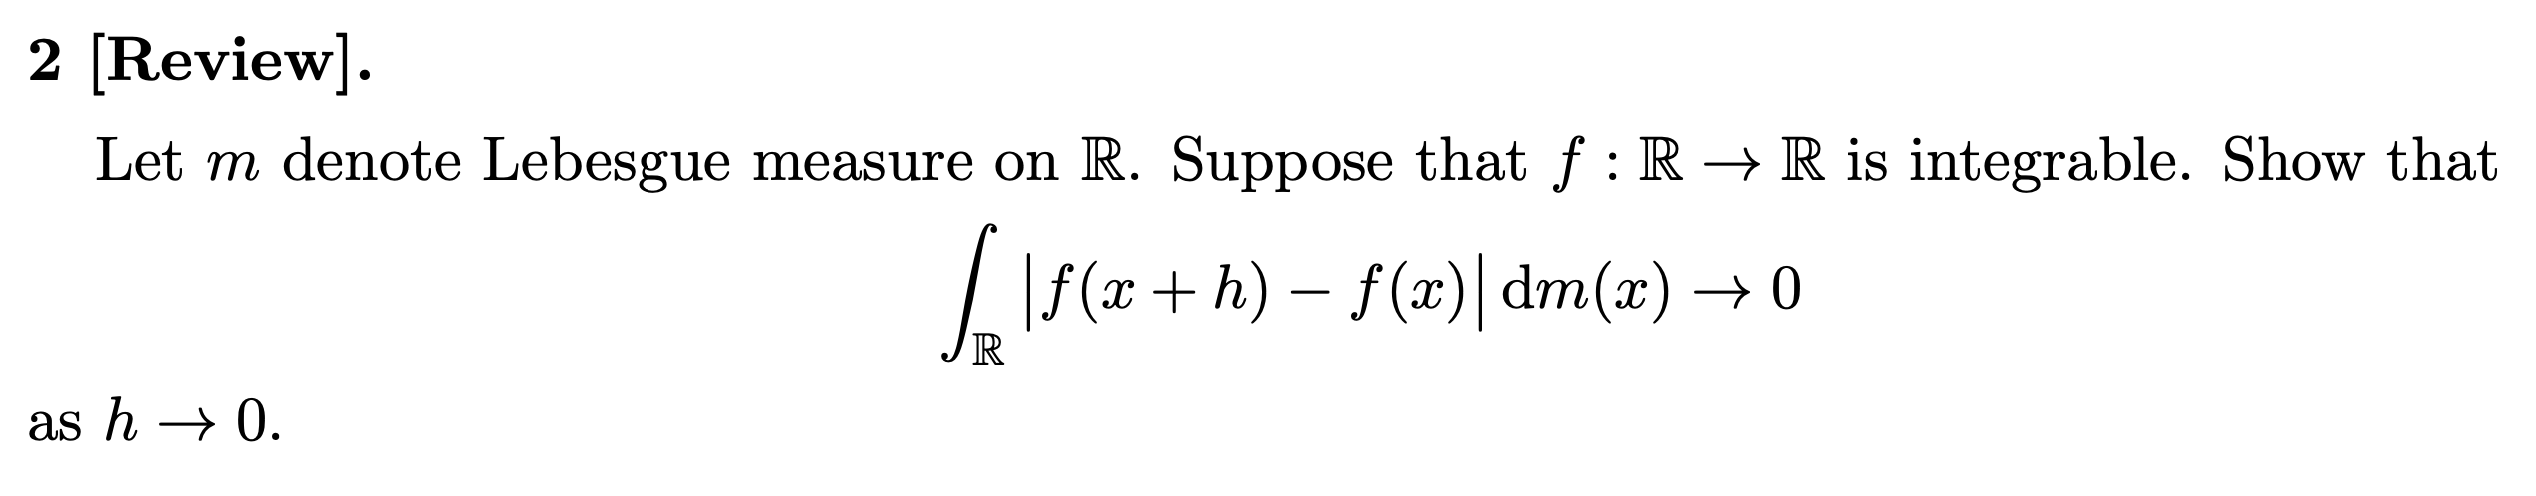
\includegraphics[width=400pt]{img/analysis--berkeley-202a-hw10-5e9e.png}
\end{mdframed}


\newpage
\begin{mdframed}
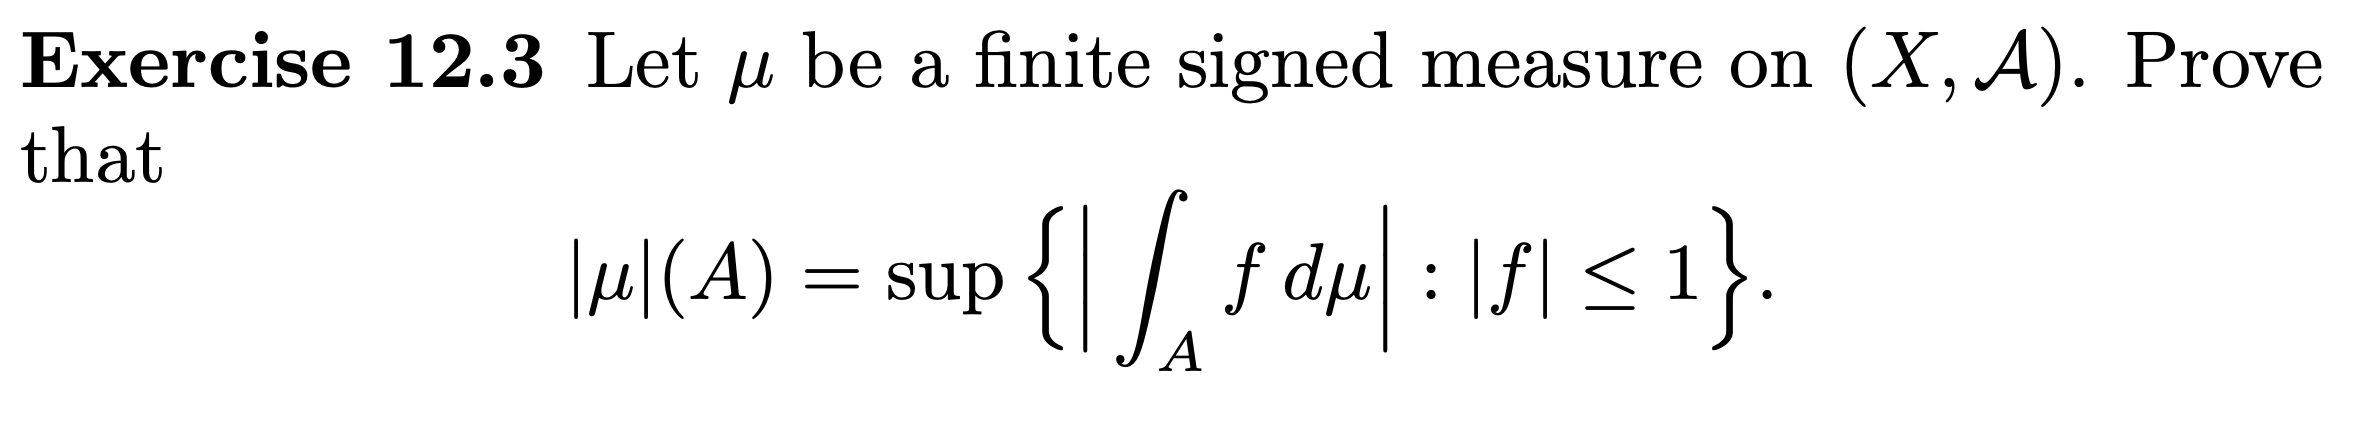
\includegraphics[width=400pt]{img/analysis--berkeley-202a-hw10-551e.png}
\end{mdframed}

\begin{intuition*}
  $|\mu|(A)$ is the total area above or below the x-axis. So it's kind of like
  \begin{align*}
    \int_M
  \end{align*}
\end{intuition*}

\begin{proof}
  We have $|\mu| := \mu^+ + \mu^-$.


\end{proof}


\newpage
\begin{mdframed}
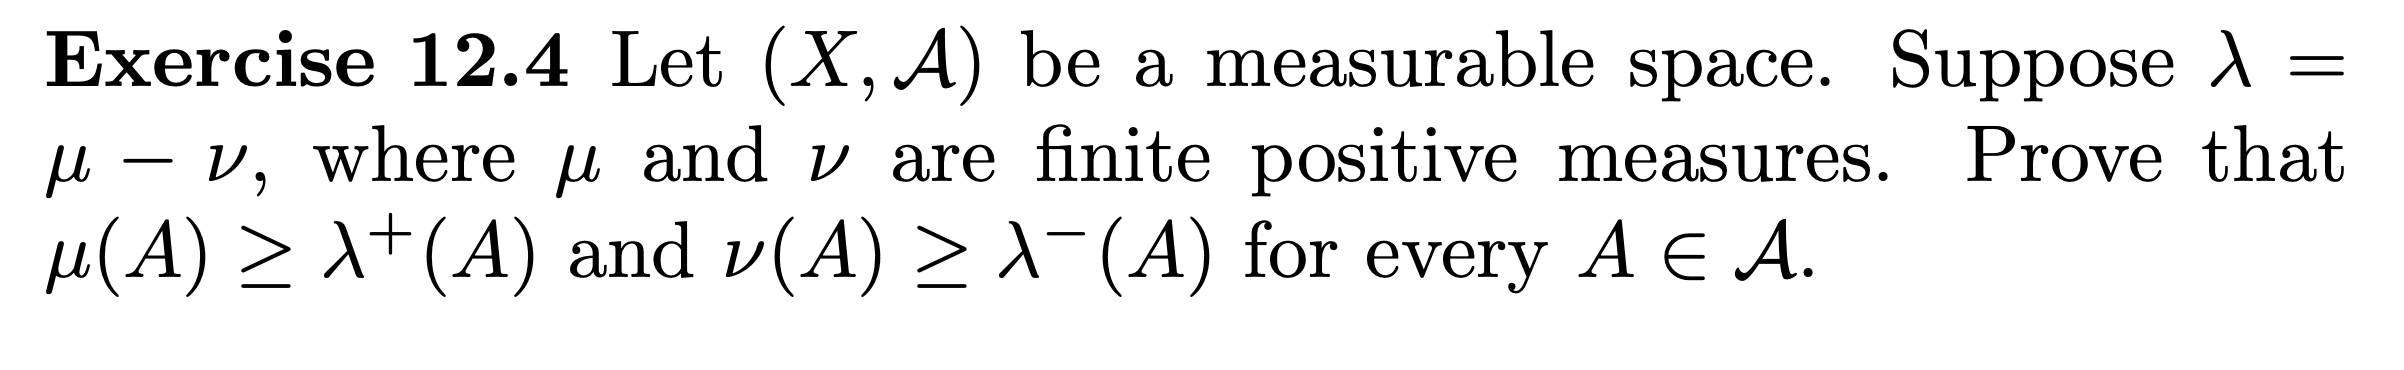
\includegraphics[width=400pt]{img/analysis--berkeley-202a-hw10-8336.png}
\end{mdframed}

\newpage
\begin{mdframed}
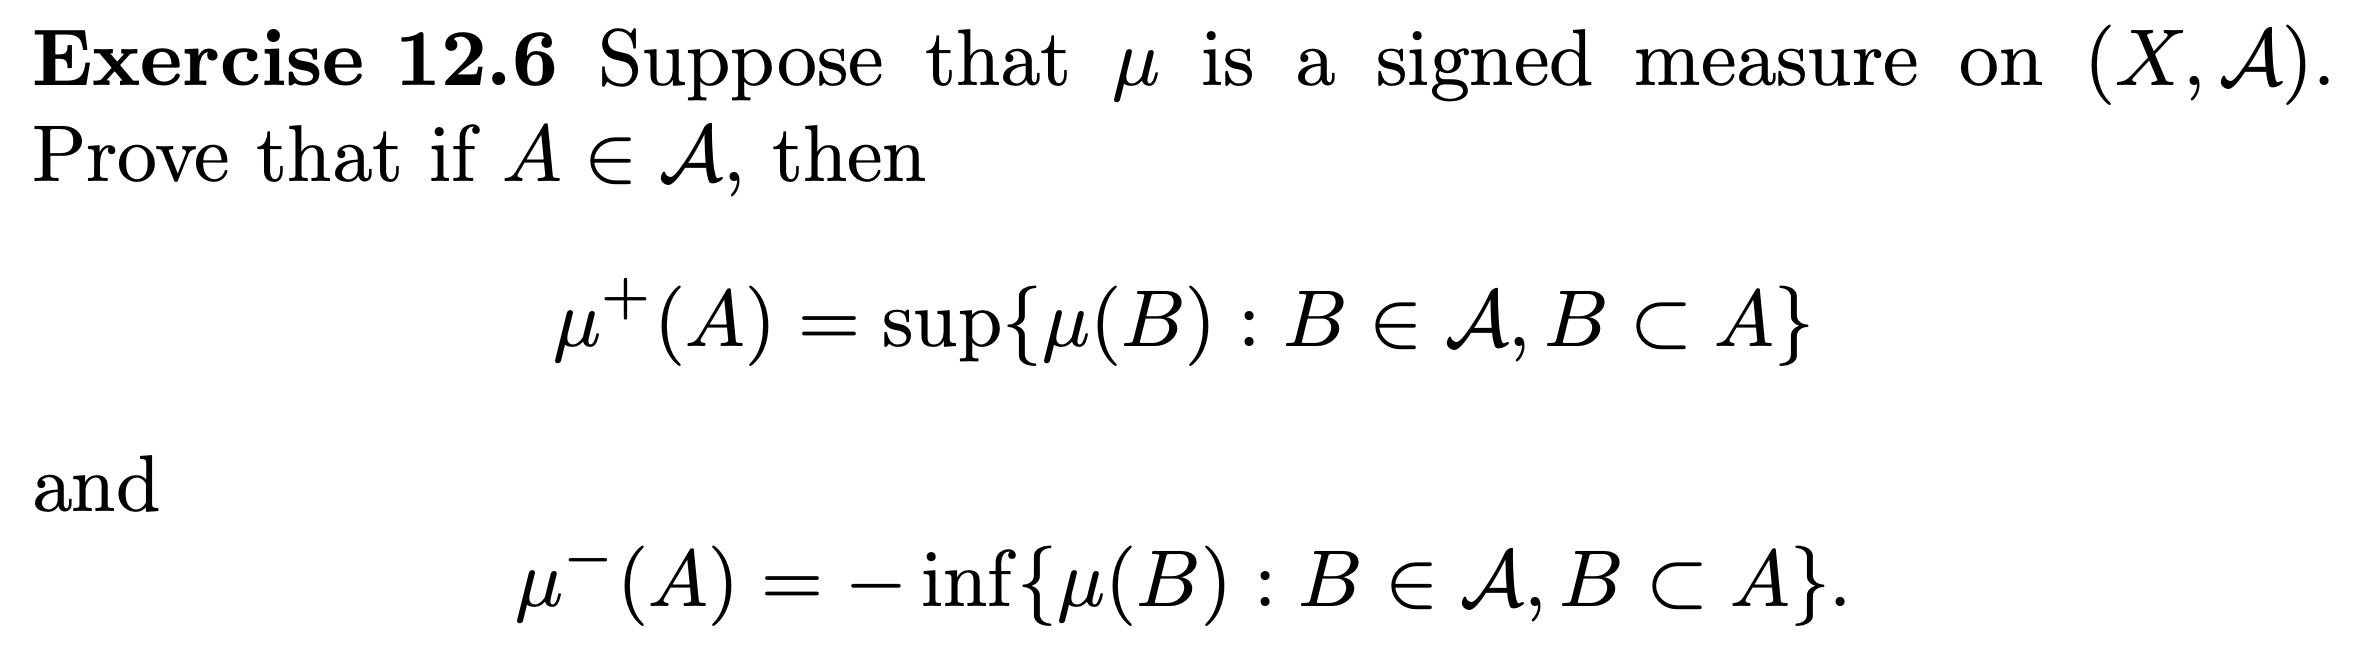
\includegraphics[width=400pt]{img/analysis--berkeley-202a-hw10-0220.png}
\end{mdframed}
